% vim:encoding=utf8 ft=tex sts=2 sw=2 et:

\documentclass{classrep}
\usepackage[utf8]{inputenc}
\usepackage{natbib} % potrzba do bibliografii
\usepackage{listings}
\usepackage{graphicx}
\usepackage{amsmath}
\usepackage{amsfonts}
\usepackage{amssymb}
\usepackage{amsthm}
\usepackage{polski}
\usepackage[hidelinks]{hyperref}
\usepackage{lmodern}  % for bold teletype font
\usepackage{amsmath}  % for \hookrightarrow
\usepackage{xcolor}   % for \textcolor
\usepackage{listings}
\usepackage{lipsum}
\usepackage{longtable}

\lstset{
  basicstyle=\ttfamily,
  columns=fullflexible,
  frame=single,
  breaklines=true,
  postbreak=\mbox{\textcolor{red}{$\hookrightarrow$}\space},
}


\newtheorem{definition}{Definicja}
\newtheorem{theorem}{Twierdzenie}

\studycycle{Informatyka, studia zaoczne, inż I st.}
\coursesemester{V}

%\coursename{Angelologia teoretyczna i stosowana}
\coursename{Sztuczna inteligencja i systemy ekspertowe}
\courseyear{2017/2018}

\courseteacher{mgr inż. Paweł Tarasiuk}
\coursegroup{sobota, 14:45}

\author{
  \studentinfo{Natalia Mateuszuk}{203940} \and
  \studentinfo{Adrian Grzelak}{200242}
}

\title{Zadanie 2 \\
Klasyfikator oparty o metodę k najbliższych sąsiadów (k-NN).}
%\svnurl{http://serce.ics.p.lodz.pl/svn/labs/atis/b_wt1415/grupa/zad1@134}

\begin{document}
\maketitle

\section{Wstęp}
Celem zadania jest zbadanie klasyfikatora opartego o metodę k najbliższych sąsiadów korzystając z dwóch zbiorów danych \citep{iris}\textit{iris} oraz \citep{wine}\textit{wine}. W tym celu metodą 3-krotnej kroswalidacji zostanie podjęta próba zaklasyfikowania każdego z elementów zbioru. Porównane ze sobą zostaną wyniki uzyskane przy pomocy różnych metryk, różnego doboru wartości $k$, po uprzednim znormalizowaniu zbioru danych jak i uprzednim jego ustandaryzowaniu. Wyniki uzyskane w sprawozdaniu zostały przy pomocy programu  \texttt{knn.exe}, który specjalnie do tego celu został stworzony.
\subsection{Klasyfikator k-NN}
Klasyfikator oparty o metodę k najbliższych sąsiadów, jest to klasyfikator, który w celu stwierdzenia przynależności obserwacji do klasy, wyszukuje w zbiorze treningowym k najbliższych dla tej obserwacji sąsiadów (Na podstawie najmniejszych odległości wg. zdefiniowanej metryki). Następnie przyporządkowuje ją do klasy, która najliczniej występowała wśród tych sąsiadów. W przypadku gdy pewne klasy występują równolicznie, wybierana jest ta która ma swój element najbliżej.
\begin{center}
	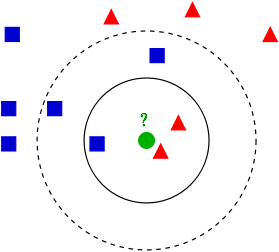
\includegraphics[height=3cm]{knn_vis.png}
	
	\textbf{Rysunek} \citep{wikipedia} W przypadku k=3, zielona kropka zostanie zakwalifikowana do czerwonych trójkątów. W przypadku k=5 natomiast do niebieskich kwadratów.
\end{center}
\subsection{Metryki}
W programie zostało zaimplementowane 5 metryk. Jednakże do naszej analizy wykorzystamy jedynie 3 (euklidesowa,manhattan,czebyszewa).
\subsubsection{Metryka Euklidesowa}
Odległość w $\mathbb{R}^n$ dla metryki euklidesowej zdefiniowana jest następująco:
\begin{equation*}
dist_e(x,y) = \sqrt{\sum_{i=1}^n (x_i - y_i)^2}
\end{equation*}
Jest to najbardziej intuicyjna metryka.

\subsubsection{Metryka Euklidesowa do kwadratu}
Odległość w $\mathbb{R}^n$ dla metryki euklidesowej do kwadratu zdefiniowana jest następująco:
\begin{equation*}
dist_{e^2}(x,y) = \sum_{i=1}^n (x_i - y_i)^2
\end{equation*}
Metryka która daje takie same wyniki przy klasyfikacji co metryka euklidesowa, jednakże ze względu na to że nie trzeba wykonywać pierwiastkowania to czas obliczeń ulega skróceniu.
\bibliographystyle{plain}

\subsubsection{Metryka Manhattan}
Odległość w $\mathbb{R}^n$ dla metryki manhattan zdefiniowana jest następująco:
\begin{equation*}
dist_m(x,y) = \sum_{i=1}^n |x_i - y_i|
\end{equation*}

\subsubsection{Metryka Czebyszewa}
Odległość w $\mathbb{R}^n$ dla metryki Czebyszewa zdefiniowana jest następująco:
\begin{equation*}
dist_cz(x,y) = \max_{i=1..n} |x_i - y_i|
\end{equation*}

\subsubsection{Metryka Minkowskiego}
Odległość w $\mathbb{R}^n$ dla metryki Minkowskiego do potęgi p zdefiniowana jest następująco:
\begin{equation*}
dist_{m^p}(x,y) = \left({\sum_{i=1}^n (x_i - y_i)^p}\right)^{\frac{1}{p}}
\end{equation*}
Można zauważyć że metryka ta jest uogólnieniem dla poprzednich metryk. dla $p=1$ jest równoważna metryce Manhattan, dla $p=2$ metryce euklidesowej, dla $p=4$ metryce euklidesowej do kwadratu i dla $p\rightarrow\infty$ metryce Czebyszewa.

\subsection{Kroswalidacja}
Sprawdzian krzyżowy to metoda statystyczna, polegająca na podziale próby statystycznej na podzbiory, a następnie przeprowadzaniu wszelkich analiz na niektórych z nich (zbiór uczący), podczas gdy pozostałe służą do potwierdzenia wiarygodności jej wyników (zbiór testowy, zbiór walidacyjny). Bez jej zastosowania nie można być pewnym czy model będzie dobrze działał dla danych, które nie były wykorzystywane do jego konstruowania (zob. overfitting).

K-krotna walidacja
W tej metodzie, oryginalna próba jest dzielona na K podzbiorów. Następnie kolejno każdy z nich bierze się jako zbiór testowy, a pozostałe razem jako zbiór uczący i wykonuje analizę. Analiza jest więc wykonywana K razy. K rezultatów jest następnie uśrednianych (lub łączonych w inny sposób) w celu uzyskania jednego wyniku.
\begin{center}
	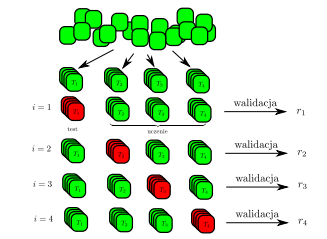
\includegraphics[height=8cm]{kros.png}
	
	\textbf{Rysunek} \citep{wikipedia} Schemat ideowy kroswalidacji
\end{center}


\subsection{Błędy pierwszego i drugiego rodzaju}
Błąd pierwszego rodzaju (błąd pierwszego typu, alfa-błąd, ang. false positive) - błąd polegający na odrzuceniu hipotezy zerowej, która w rzeczywistości nie jest fałszywa. Oszacowanie prawdopodobieństwa popełnienia błędu pierwszego rodzaju oznaczamy symbolem $\alpha$ (mała grecka litera alfa) i nazywamy poziomem istotności testu. Termin false positive jest często używany w odniesieniu do oprogramowania antywirusowego, które omyłkowo klasyfikuje zdrowy plik jako zainfekowany.
Błąd drugiego rodzaju (błąd drugiego typu, błąd przyjęcia, beta-błąd, ang. false negative) - błąd polegający na nieodrzuceniu hipotezy zerowej, która jest w rzeczywistości fałszywa.
Oszacowanie prawdopodobieństwa popełnienia błędu drugiego rodzaju oznaczamy symbolem $\beta$ (mała grecka litera beta), a jego dopełnienie do jedności nazywane jest mocą testu. W odniesieniu do oprogramowania antywirusowego, błąd drugiego rodzaju polega na niewykryciu szkodliwego kodu. Innymi słowy, zainfekowany plik uznawany jest za bezpieczny. W przypadku diagnoz medycznych, błąd drugiego rodzaju oznacza brak rozpoznania choroby u pacjenta. Tzn. pomimo występowania schorzenia, pacjent nie zostaje rozpoznany względem danego schorzenia.


Prawdopodobieństwo popełnienia błędu drugiego rodzaju wiąże się z tzw. mocą testu statystycznego i oznaczony jest mała grecką literą beta. Moc testu to 1 minus Beta. Błąd I i II rodzaju są ze sobą ściśle powiązane: im częściej odrzucana będzie hipoteza zerowa tym większe ryzyko popełnienia błędu I rodzaju, ale mniejsze ryzyko popełnienia błędu II rodzaju. Z kolei jeśli będziemy bardziej restrykcyjni w poszukiwaniu dowodów na to, że hipoteza zerowa jest nieprawdziwa (nie będziemy jej tak łatwo odrzucać) to oczywiście spada prawdopodobieństwo popełnienia błędu I rodzaju, ale rośnie prawdopodobieństwo popełnienia II rodzaju czyli tzw. moc testu spada.

\begin{center}
	
\includegraphics[height=4cm]{bledy.png}
	
	\textbf{Rysunek} \citep{wikipedia} Tabela Błędów I i II rodzaju
\end{center}



\section{Wyniki}
\subsection{Tabela wyników}
\begin{center}
\begin{longtable}{|r|r|r|r|r|r|}
  \hline 
  Zbiór Danych & Metryka & k & Normalizacja & Standaryzacja & Trafność \\
	\hline
		iris & Euclidean & 1 & no & no & 96.00\% \\
	\hline
		iris & Euclidean & 3 & no & no & 96.67\% \\
	\hline
		iris & Euclidean & 5 & no & no & 95.33\% \\
	\hline
		iris & Euclidean & 10 & no & no & 96.00\% \\
	\hline
		iris & Euclidean & 1 & yes & no & 96.00\% \\
	\hline
		iris & Euclidean & 3 & yes & no & 95.33\% \\
	\hline
		iris & Euclidean & 5 & yes & no & 96.00\% \\
	\hline
		iris & Euclidean & 10 & yes & no & 96.67\% \\
	\hline
		iris & Euclidean & 1 & no & yes & 94.00\% \\
	\hline
		iris & Euclidean & 3 & no & yes & 94.67\% \\
	\hline
		iris & Euclidean & 5 & no & yes & 95.33\% \\
	\hline
		iris & Euclidean & 10 & no & yes & 96.67\% \\
	\hline
		iris & Manhattan & 1 & no & no & 96.00\% \\
	\hline
		iris & Manhattan & 3 & no & no & 96.00\% \\
	\hline
		iris & Manhattan & 5 & no & no & 94.67\% \\
	\hline
		iris & Manhattan & 10 & no & no & 95.33\% \\
	\hline
		iris & Manhattan & 1 & yes & no & 94.67\% \\
	\hline
		iris & Manhattan & 3 & yes & no & 94.67\% \\
	\hline
		iris & Manhattan & 5 & yes & no & 94.67\% \\
	\hline
		iris & Manhattan & 10 & yes & no & 95.33\% \\
	\hline
		iris & Manhattan & 1 & no & yes & 93.33\% \\
	\hline
		iris & Manhattan & 3 & no & yes & 95.33\% \\
	\hline
		iris & Manhattan & 5 & no & yes & 94.00\% \\
	\hline
		iris & Manhattan & 10 & no & yes & 95.33\% \\
	\hline
		iris & Chebyshev & 1 & no & no & 96.67\% \\
	\hline
		iris & Chebyshev & 3 & no & no & 96.00\% \\
	\hline
		iris & Chebyshev & 5 & no & no & 98.00\% \\
	\hline
		iris & Chebyshev & 10 & no & no & 98.00\% \\
	\hline
		iris & Chebyshev & 1 & yes & no & 95.33\% \\
	\hline
		iris & Chebyshev & 3 & yes & no & 96.00\% \\
	\hline
		iris & Chebyshev & 5 & yes & no & 96.00\% \\
	\hline
		iris & Chebyshev & 10 & yes & no & 96.67\% \\
	\hline
		iris & Chebyshev & 1 & no & yes & 94.00\% \\
	\hline
		iris & Chebyshev & 3 & no & yes & 94.67\% \\
	\hline
		iris & Chebyshev & 5 & no & yes & 96.00\% \\
	\hline
		iris & Chebyshev & 10 & no & yes & 95.33\% \\
	\hline
	\hline
		wine & Euclidean & 1 & no & no & 74.16\% \\
	\hline
		wine & Euclidean & 3 & no & no & 68.54\% \\
	\hline
		wine & Euclidean & 5 & no & no & 73.60\% \\
	\hline
		wine & Euclidean & 10 & no & no & 73.60\% \\
	\hline
		wine & Euclidean & 1 & yes & no & 95.51\% \\
	\hline
		wine & Euclidean & 3 & yes & no & 96.63\% \\
	\hline
		wine & Euclidean & 5 & yes & no & 97.19\% \\
	\hline
		wine & Euclidean & 10 & yes & no & 96.63\% \\
	\hline
		wine & Euclidean & 1 & no & yes & 95.51\% \\
	\hline
		wine & Euclidean & 3 & no & yes & 95.51\% \\
	\hline
		wine & Euclidean & 5 & no & yes & 96.63\% \\
	\hline
		wine & Euclidean & 10 & no & yes & 97.19\% \\
	\hline
		wine & Manhattan & 1 & no & no & 81.46\% \\
	\hline
		wine & Manhattan & 3 & no & no & 76.97\% \\
	\hline
		wine & Manhattan & 5 & no & no & 78.65\% \\
	\hline
		wine & Manhattan & 10 & no & no & 79.21\% \\
	\hline
		wine & Manhattan & 1 & yes & no & 97.19\% \\
	\hline
		wine & Manhattan & 3 & yes & no & 97.19\% \\
	\hline
		wine & Manhattan & 5 & yes & no & 98.31\% \\
	\hline
		wine & Manhattan & 10 & yes & no & 98.31\% \\
	\hline
		wine & Manhattan & 1 & no & yes & 97.75\% \\
	\hline
		wine & Manhattan & 3 & no & yes & 97.19\% \\
	\hline
		wine & Manhattan & 5 & no & yes & 97.75\% \\
	\hline
		wine & Manhattan & 10 & no & yes & 97.75\% \\
	\hline
		wine & Chebyshev & 1 & no & no & 69.10\% \\
	\hline
		wine & Chebyshev & 3 & no & no & 68.54\% \\
	\hline
		wine & Chebyshev & 5 & no & no & 73.03\% \\
	\hline
		wine & Chebyshev & 10 & no & no & 71.35\% \\
	\hline
		wine & Chebyshev & 1 & yes & no & 93.26\% \\
	\hline
		wine & Chebyshev & 3 & yes & no & 96.07\% \\
	\hline
		wine & Chebyshev & 5 & yes & no & 93.82\% \\
	\hline
		wine & Chebyshev & 10 & yes & no & 94.94\% \\
	\hline
		wine & Chebyshev & 1 & no & yes & 94.94\% \\
	\hline
		wine & Chebyshev & 3 & no & yes & 93.82\% \\
	\hline
		wine & Chebyshev & 5 & no & yes & 93.82\% \\
	\hline
		wine & Chebyshev & 10 & no & yes & 94.38\% \\


  \hline
\end{longtable} 
\textbf{Tabela.} Wyniki dla eksperymentów
\end{center}

dla zbioru iris najlepsze wyniki trafności zostały osiągnięte przy stosowaniu metryki Chebysheva, bez stosowania standaryzacji i normalizacji. Dla zbioru wine najlepsze wyniki trafności zostały osiągnięte przy stosowaniu metryki Manhattan, z zastosowaniem normalizacji. Najlepsze wyniki osiągano dla k równego 5 lub 10. Na poniższym obrazku możemy zobaczyć stopień skorelowania pomiędzy poszczególnymi parametrami.

\begin{center}
	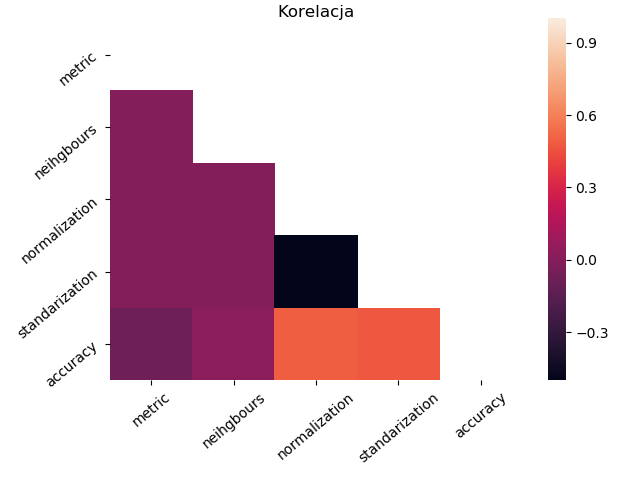
\includegraphics[height=8cm]{korelacja.png}
	
	\textbf{Rysunek} Skorelowanie pomiędzy wynikami a parametrami testu dla zbioru danych wine
\end{center}

Od razu rzuca się w oczy że zastosowanie normalizacji ma największy pozytywny wpływ na uzyskaną skuteczność (Silnie dodatnio skorelowana). Na drugim miejscu zaraz za nią plasuje się standaryzacja. Zastosowane liczba sąsiadów $k$ oraz metryka mają również wpływ jednakże nie tak znaczny. Warto zatem przy klasyfikowaniu metodą kNN zastosować normalizację wprowadzanych danych. Warto również pokusić się o sprawdzenie optymalnej liczby sąsiadów. Zbyt mała może przekłamywać niektóre wyniki, podobnie zbyt duża. Sprawdzenie różnych metryk również jest wskazane - na przykładzie naszych zbiorów danych widać, że dla irysów najlepsze wyniki mamy w metryce Czebyszewa, tymczasem dla win w metryce Manhattan.

\subsection{Przykładowy test dla iris}
\begin{verbatim}
==================INFO ABOUT TEST=================
File: iris.data ,Attributes: 4 ,Instances: 150
Classes: Iris-setosa, Iris-versicolor, Iris-virginica
Method: 3-fold cross-validation
Metric: Euclidean
Nearest neighbours checked: 1
Standarized=no ,Normalization=no
Computing time: 17ms
===================TEST RESULTS===================
Error Matrix:
  50    0    0   | Iris-setosa
   0   47    3   | Iris-versicolor
   0    3   47   | Iris-virginica
Statistics:
 False Positive Ratio (I):
   Iris-setosa - 0.00% (0)
   Iris-versicolor - 6.00% (3)
   Iris-virginica - 6.00% (3)
 False Negative Ratio (II):
   Iris-setosa - 0.00% (0)
   Iris-versicolor - 6.00% (3)
   Iris-virginica - 6.00% (3)
 Accuracy: 96.00%
\end{verbatim}

pierwsza grupa testowa ze zbioru irysy podlega bardzo dobrej klasyfikacji, grupa 2 i 3 kwiatów prawdopodobnie jest podobna ponieważ następują pewne pomyłki w klasyfikacji.

\subsection{Przykladowy test dla wine}

\begin{verbatim}
==================INFO ABOUT TEST=================
File: wine.data ,Attributes: 13 ,Instances: 178
Classes: 1, 2, 3
Method: 3-fold cross-validation
Metric: Euclidean
Nearest neighbours checked: 5
Standarized=no ,Normalization=no
Computing time: 56ms
===================TEST RESULTS===================
Error Matrix:
  56    0    3   | 1
   4   49   18   | 2
   3   19   26   | 3
Statistics:
 False Positive Ratio (I):
   1 - 11.11% (7)
   2 - 27.94% (19)
   3 - 44.68% (21)
 False Negative Ratio (II):
   1 - 5.08% (3)
   2 - 30.99% (22)
   3 - 45.83% (22)
 Accuracy: 73.60%
\end{verbatim}

pierwsza grupa testowa ze zbioru win podlega bardzo dobrej klasyfikacji, grupa 2 i 3 win prawdopodobnie jest podobna ponieważ następują pewne pomyłki w klasyfikacji. W grupie 2 i 3 występuje pewne podobieństwo do grupy 1.

\bibliography{bibliografia}

\end{document}

